\documentclass[aps,pra,twocolumn]{revtex4-1}

\usepackage{graphicx,epstopdf}
\usepackage{amsmath}
\usepackage{mathrsfs}
\usepackage{mathtools}


\begin{document}


\title{Determining the drag coefficient of the mirage rocket}

\author{Evan Anders}
\author{Andrew French}
\author{John Hoff}
\author{Michael Woodkey}
\affiliation{Department of Physics, Whitworth University, 300 W. Hawthorne Rd., Spokane, WA 99251}


\date{\today}

\begin{abstract}
Abstract goes here
\end{abstract}



\maketitle


\section{\label{section1} Introduction}
In introductory physics we learned to roughly model projectile motion using gravitational forces and initial velocities.  In advanced dynamics, our understanding of the motion of objects moving through fluids has become more intricate.  We learned about linear and quadratic drag forces, the former of which arises from the viscosity of the liquid and the latter of which arises from the necessity of the projectile to push the medium out of its path.

While learning about these topics in a classroom setting is beneficial to our knowledge, it is our goal here to prove that this more accurate model applies to real data.  We were given a rocket, the Mirage, and tasked with finding the drag coefficient of that rocket.  Here we show, through calibration of motor impulse and analysis of actual flight data, the derivation of our rocket's drag coefficient.



\section{\label{section 2} Theory}
It is a good approximation to assume that drag force acts in a direction opposite to that of velocity, that is,
\begin{equation}
\vec{f}_\text{drag} = - f(v) \hat{v}.
\end{equation}
At low speeds, it is a good approximation to assume that
\begin{equation}
f(v) = b v + c v^2 = f_\text{linear} + f_\text{quadratic},
\end{equation}
where $f_\text{linear}$ arises as a result of the viscous properties of the medium through which the projectile moves and $f_\text{quadratic}$ arises from the projectile accelerating the fluid medium out of its path \cite{taylor2005}.  At high speeds, the quadratic term becomes significantly more important than the linear term, such as in the case of a rocket being rapidly propelled by a motor.  For a long, cylindrical object with a velocity aligned with the area vector of the top cylinder, we can approximate the value of the quadratic drag coefficient, such that
\begin{equation}
c = \nu A = \nu \pi r^2.
\end{equation}

For such a system, our equations of motion become \cite{taylor2005}
\begin{equation}
m \vec{\dot{v}} = m \vec{g} - c v \vec{v}
\end{equation}
Which, when examined in a 2-dimensional plane, becomes
\begin{equation}
m \dot{v}_x  = -c\sqrt{v_x^2 + v_y^2}v_x \label{xafter}
\end{equation}
and
\begin{equation}
m \dot{v}_y  = -c\sqrt{v_x^2 + v_y^2}v_y - mg. \label{yafter}
\end{equation}
While this system of equations is accurate for a rocket in motion \emph{after} its motor finishes providing thrust.  Before this time, the rocket motor provides an additional force in the direction of motion, such that
\begin{equation}
\vec{f}_\text{burn} = f_\text{burn} \hat{v}.
\end{equation}
Additionally, during this time, the mass of the rocket-motor system is decreasing.  As such, our equations of motion during the thrust of the rocket are
\begin{equation}
m(t) \dot{v}_x  = -c\sqrt{v_x^2 + v_y^2}v_x + f_\text{burn} \frac{v_x}{\sqrt{v_x^2 + v_y^2}} \label{xbefore}
\end{equation}
and
\begin{equation}
m(t) \dot{v}_y  = -c\sqrt{v_x^2 + v_y^2}v_y - m(t)g + f_\text{burn} \frac{v_y}{\sqrt{v_x^2 + v_y^2}}, \label{ybefore}
\end{equation}
whereas  the equations of motion after the thrust are, as we saw above, Eqs. (\ref{xafter}) and (\ref{yafter}), where $m = m_\text{rocket}$, which is the mass of the rocket and the spent motor.  In our equations of motion during the motor thrust, we define
\begin{equation}
m(t) = m_\text{rocket} + m_\text{fuel} \frac{t_\text{fuel} - t}{t_\text{fuel}}.
\end{equation}
With all of these pieces, we are capable of numerically solving for a value of $c$.

\begin{equation}
m(t) \dot{v}_x = 
\begin{cases}
-c\sqrt{v_x^2 + v_y^2}v_x + f_\text{burn} \frac{v_x}{\sqrt{v_x^2 + v_y^2}}, & \text{if } t < t_\text{burn} \\
-c\sqrt{v_x^2 + v_y^2}v_x, & \text{if } t >= t_\text{burn}
\end{cases}
\end{equation}


\section{\label{section 3} Calibration}
\begin{figure} [t!]
	\includegraphics[width=3in]{calibration_Plot.eps}
	\caption{\label{calibrationPlot}}
\end{figure}
\begin{figure} [b!]
	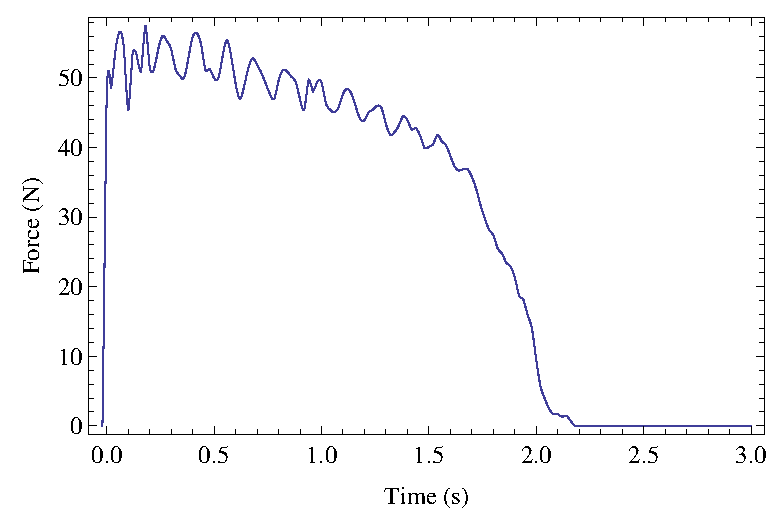
\includegraphics[width=3in]{G38-scaledTest.eps}
	\caption{\label{thrustPlot}}
\end{figure}

We created an apparatus with a system of pulleys which held up a cylindrical fitting for a rocket motor.  This motor was designed to fire upward such that force was directed downward, and wires connecting to the fitting also connected to a dual-range force sensor after encountering a system of pulleys.  In order to calibrate our apparatus, we loaded a mass hanger onto the system, zeroed our force sensor, and added weight to the hanger at increments of 0.5 kg.  A plot of force measured in the force sensor vs. force measured in the hanger can be see in Fig. \ref{calibrationPlot}.  Our best fit line for these data points shows that,
\begin{equation}
F_\text{measured} = \chi F_\text{applied} + \beta ,
\end{equation}
where $\chi = 0.0316$ and $\beta = 0.00794$, a small offset resulting from the fact that, even when zeroed, our testing apparatus did not read \emph{exactly} 0.

Using these results, we measured the force produced by a g38 motor, and applied the scaling factor, $F_\text{applied} = F_\text{measured}/\chi$ in order to find how much force, $F_\text{applied}$, the rocket motor provided.  The scaled data of the rocket motor thrust can be see in Fig. \ref{thrustPlot}. 



\section{\label{section 4} Experimental Data and Analysis}
\begin{figure} [b!]
	\includegraphics[width=3in]{Mirage-G38-BestFit.eps}
	\caption{\label{experiment}}
\end{figure}

We used the system of equations defined by Eqs. (\ref{xbefore}, \ref{xafter}, \ref{ybefore}, \ref{yafter}).


\section{\label{section 5} Conclusion}


\bibliography{Bibliography}

\end{document}